\documentclass{article}
\usepackage{geometry}
\geometry{a4paper, portrait, margin=1.5cm}
\usepackage{graphicx}
\graphicspath{ {images/} }
\usepackage{listings}
\usepackage{xcolor}

\definecolor{codegreen}{rgb}{0,0.6,0}
\definecolor{codegray}{rgb}{0.5,0.5,0.5}
\definecolor{codepurple}{rgb}{0.58,0,0.82}
\definecolor{backcolour}{rgb}{1,1,1}

\lstdefinestyle{mystyle}{
    backgroundcolor=\color{backcolour},   
    commentstyle=\color{codegreen},
    keywordstyle=\color{magenta},
    numberstyle=\tiny\color{codegray},
    stringstyle=\color{codepurple},
    basicstyle=\ttfamily\footnotesize,
    breakatwhitespace=false,  
    frame=shadowbox,       
    breaklines=true,                 
    captionpos=b,                    
    keepspaces=true,                 
    numbers=left,                    
    numbersep=5pt,                  
    showspaces=false,                
    showstringspaces=false,
    showtabs=false,                  
    tabsize=2
}
    
\lstset{style=mystyle}

\author{\Large submitted by\\ Arghya Bandyopadhyay\\
    	RollNo. 20CS4103\\}
\title{\begin{center}
       \bfseries\Large
    	Assignment 4\\
    	Of\\
    	Network \& Distributed System Lab (CS2051)\\
        Masters of Technology in Computer Science And Engineering\\
    	\vskip1cm
    	submitted to\\
    	Dr Sujoy Saha\\
    	Assistant Professor\\
    	Dept. of CSE\\
    	\vskip1cm
    	
\includegraphics[width=4cm]{NITDGP}\\
    	National Institute of Technology, Durgapur\\
    \end{center}}
\date{1 Jul 2021}
\begin{document}
\maketitle
\pagebreak

\textbf{Objective:} Sync is a communication protocol for peer-to-peer file sharing (P2P), enabling users to distribute data and electronic files over the Internet/offline in a decentralized manner. 

Design and Implement a sync protocol using “nanohttpd” which will transfer multimodal files (Text, Image, Audio, and Video), and if the connection is intermittent during the synching, the process can restart the services and resume the cycle/process.

\begin{figure}[ht]
\centering
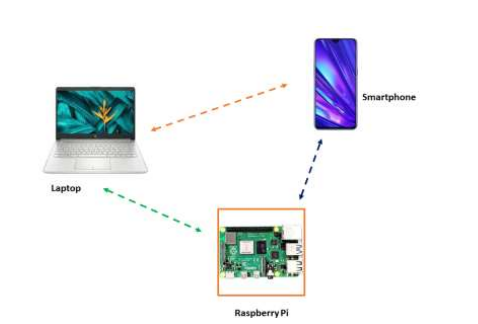
\includegraphics[width=350pt]{Question1Diagram1}
\caption{Information exchange between heterogeneous nodes}
\label{fig:Question1Diagram1}
\end{figure}

\begin{figure}[ht]
\centering
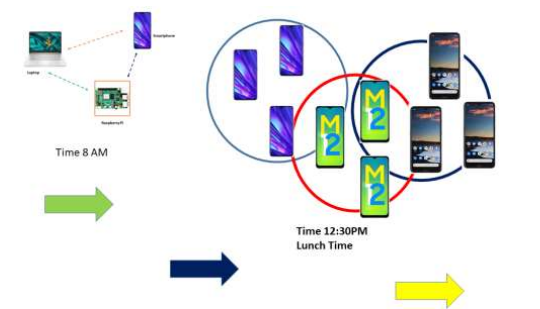
\includegraphics[width=350pt]{Question1Diagram2}
\caption{File synching (store and forwarding approach) between the nodes and file can move from
one place another due to the movement of the nodes.}
\label{fig:Question1Diagram2}
\end{figure}

\pagebreak
\begin{flushleft}
\textbf{Answer.}

\textbf{$build.gradle$}
\lstinputlisting[language=xml]{listedCodes/build.gradle}
\textbf{$activity\_main.xml$}
\lstinputlisting[language=xml]{listedCodes/activity_main.xml}
\textbf{$AndroidManifest.xml$}
\lstinputlisting[language=xml]{listedCodes/AndroidManifest.xml}
\textbf{$GetFileExtension.java$}
\lstinputlisting[language=java]{listedCodes/GetFileExtension.java}
\textbf{$Download.java$}
\lstinputlisting[language=java]{listedCodes/Download.java}
\textbf{$Ip.java$}
\lstinputlisting[language=java]{listedCodes/Ip.java}
\textbf{$Main.java$}
\lstinputlisting[language=java]{listedCodes/Main.java}
\textbf{$MainActivity.java$}
\lstinputlisting[language=java]{listedCodes/MainActivity.java}
\end{flushleft}

\textbf{Output:}

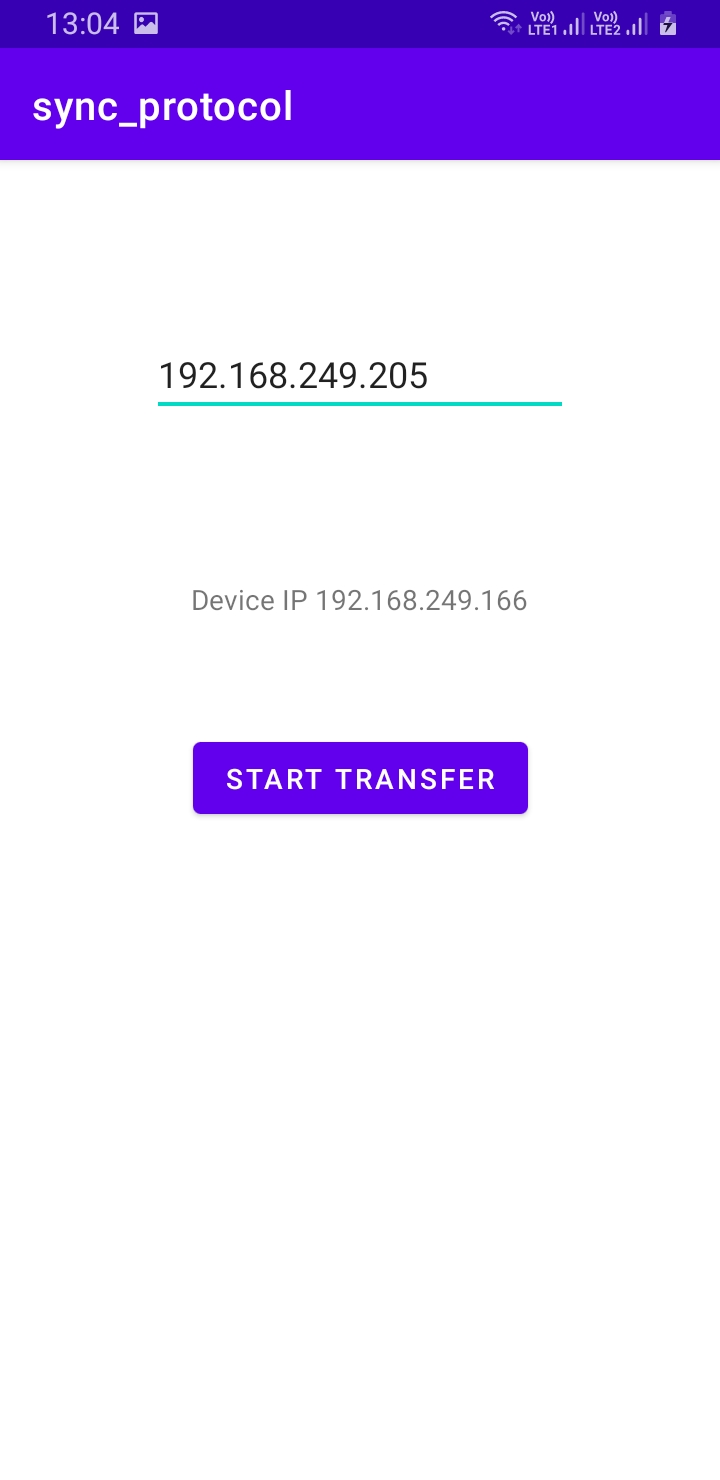
\includegraphics[height=350pt]{Output1}
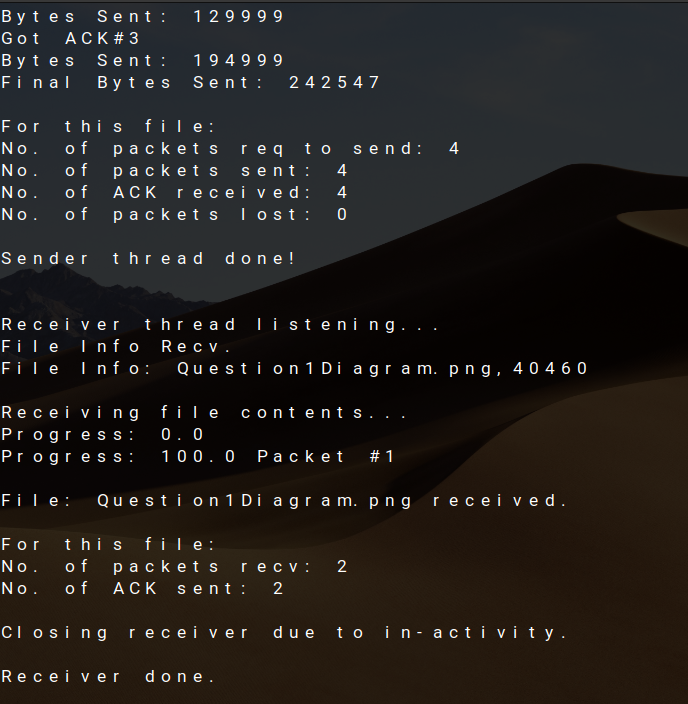
\includegraphics[height=350pt]{Output2}
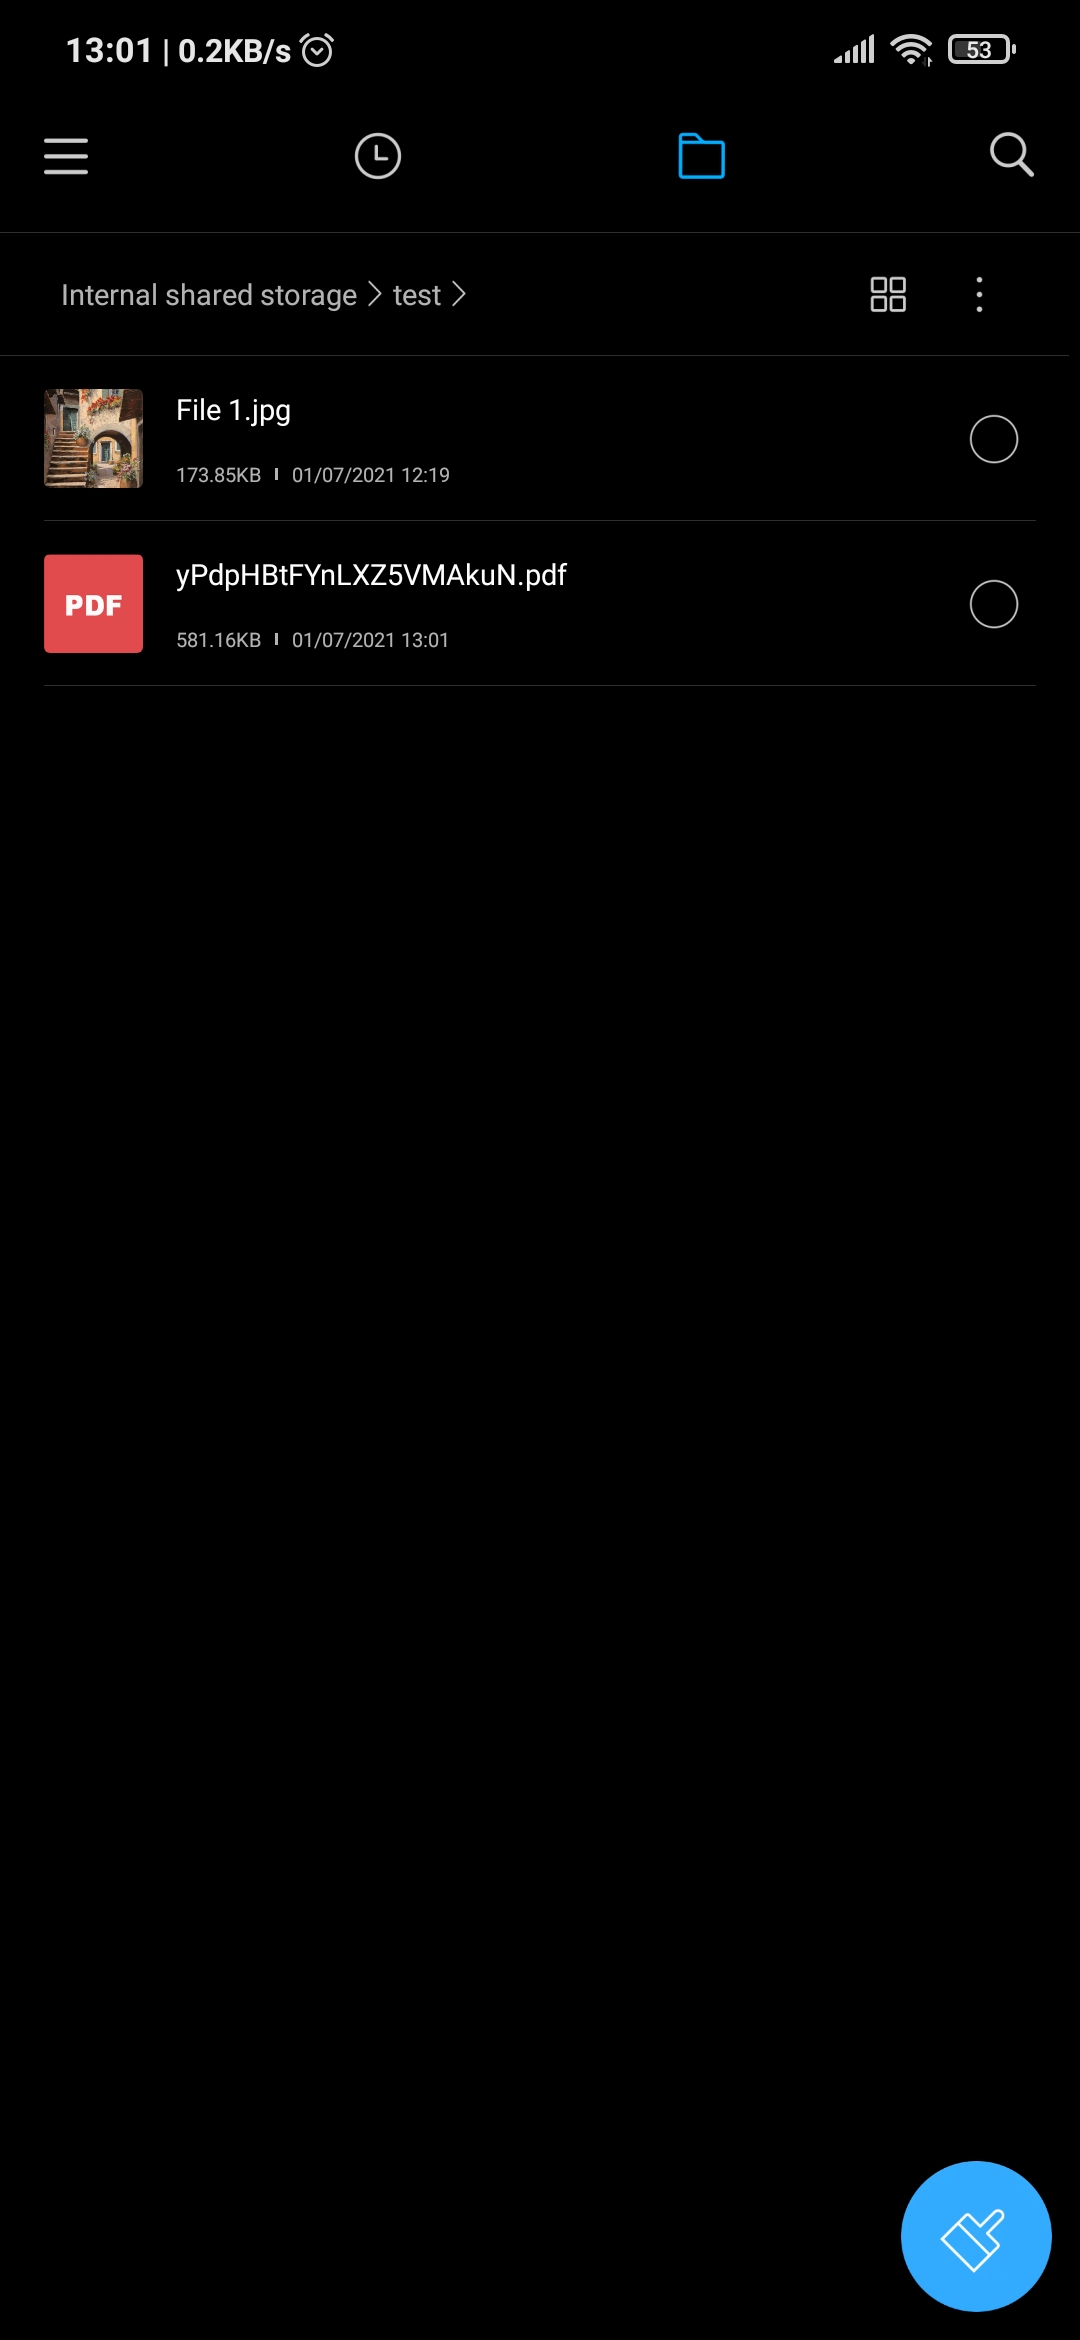
\includegraphics[height=350pt]{Output3}

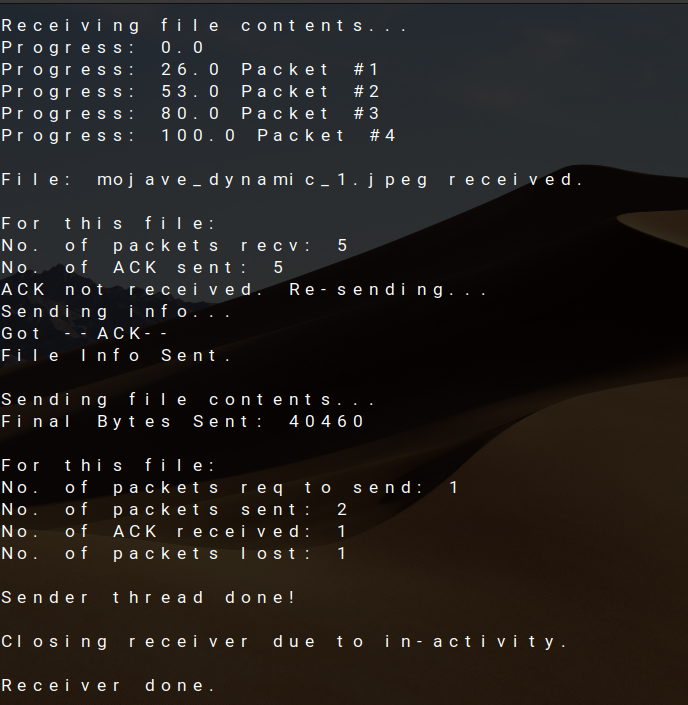
\includegraphics[height=350pt]{Output4}
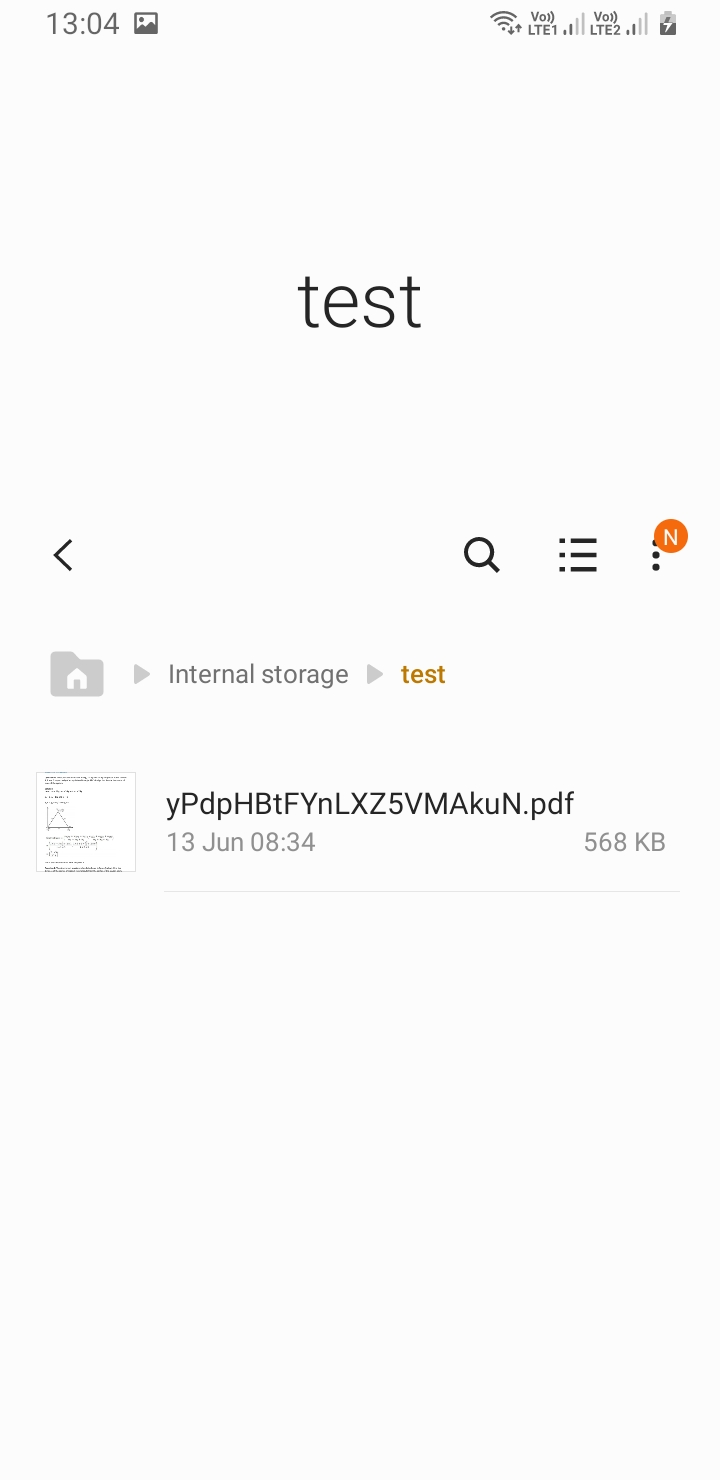
\includegraphics[height=350pt]{Output5}
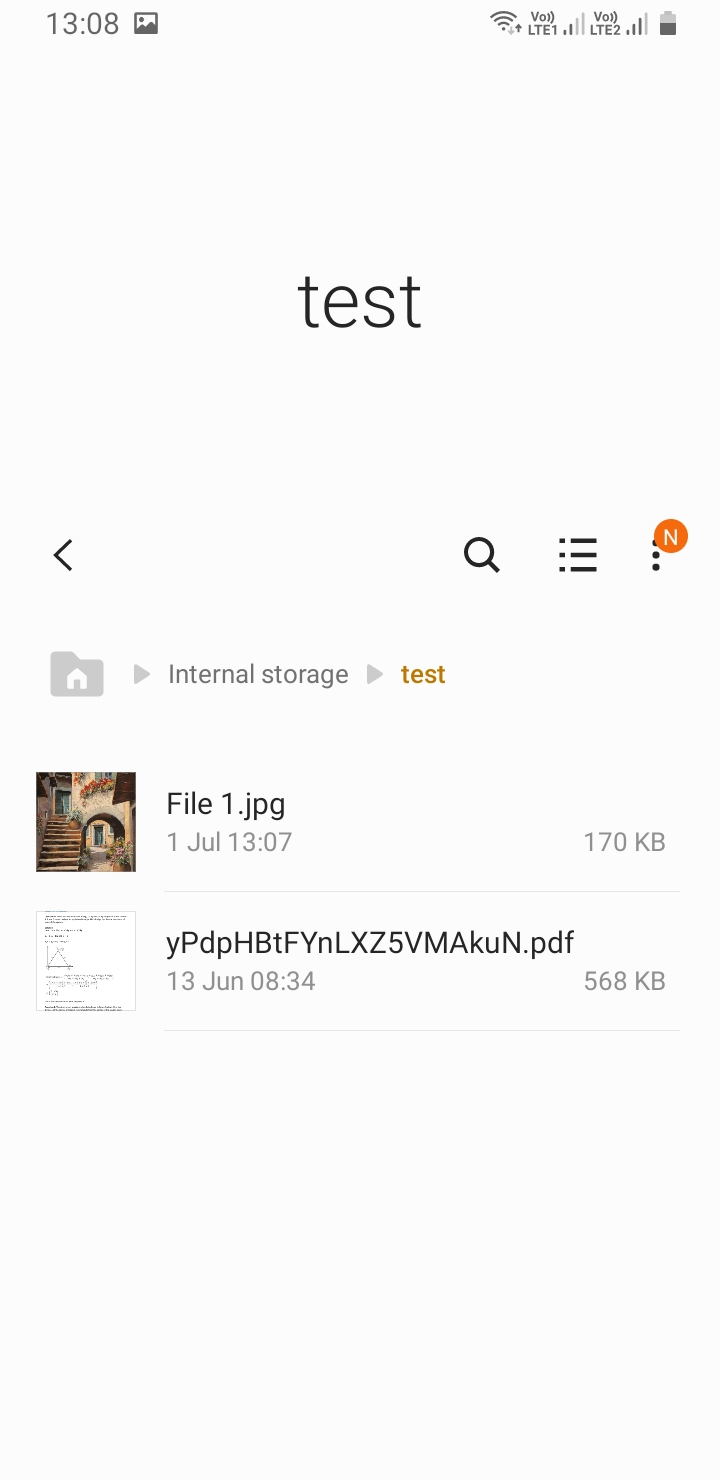
\includegraphics[height=350pt]{Output6}
\end{document}
